\section{Verkáætlun}
Hér skal gera verkáætlun og tímaáætlun, setja in mynd af henni gerð í https://draw.io veljið Flocharts-gant .  þegar þið hafið lokið við grafið farið í export-image og vistið sem `gant` í skyrsla/img

Fyrir þetta verkefni höfum við u.þ.b þrjá mánuði til stefnu. Hingað til höfum við verið að mestu leiti að vinna í fræðilega hluta verkefnisins.  Við höfum verið að vinna í og semja verkefna lýsinguna, ákveða hvaða hluti og íhluti þarf og síðan höfum við nýlega verið að vinna í því að tengja arduinio uno tölvuna við motor.  Næsta skrefið væri að kynna okkur og prufa okkur áfram með þrýstinema ætti að taka u.þ.b eina kennslustund. Síðan þurfum við að vinna með þrýstinemann og gera útreikninga og áætla hvernig við ætlum að vinna með þyngdarbreyturnar. Eftir það væri hægt að fíngera kóðann og gera breytingar þannig að t.d í staðinn fyrir að opna hliðið þegar að skálin fer undir ákveðið þyngdarstig myndi það opnast t.d einu sinni á dag á ákveðnum tíma. Síðan myndum við smíða vélmennið og breyta eftir þörfum.
\begin{figure}[h]
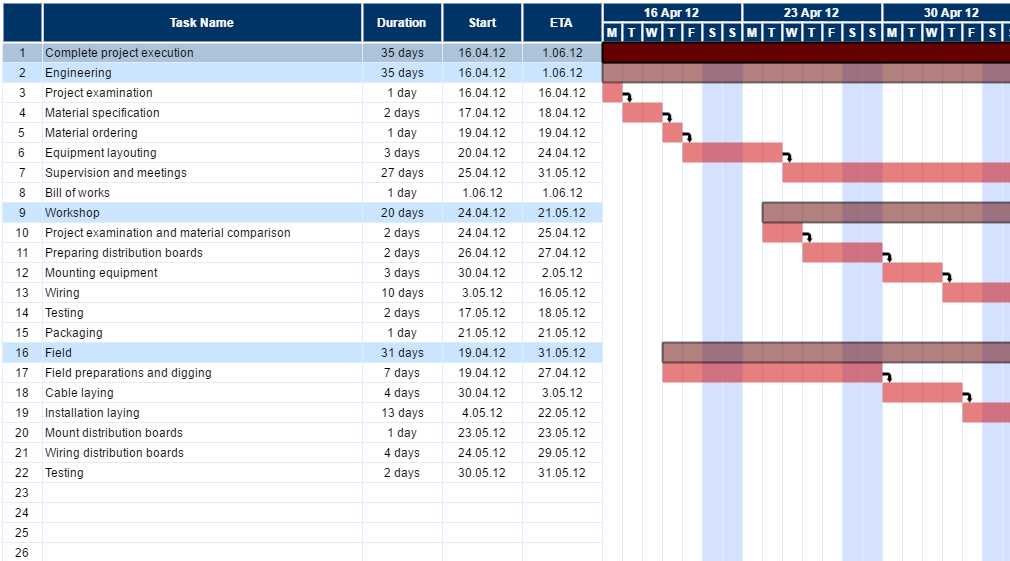
\includegraphics[scale=.3]{img/gant}
\end{figure}